\documentclass[11pt, a4paper, twoside]{article}

% Version en 2024 Víctor Bettachini < vbettachini@unlam.edu.ar >

\usepackage[T1]{fontenc}
\usepackage[utf8]{inputenc}

% \usepackage[spanish, es-tabla]{babel}
% \def\spanishoptions{argentina} % Was macht dass?
% \usepackage{babelbib}
% \selectbiblanguage{spanish}
% \addto\shorthandsspanish{\spanishdeactivate{~<>}}

\usepackage{graphicx}
\graphicspath{{../figuresLaTeX/}}
% \usepackage{float}

\usepackage[arrowdel]{physics}
\newcommand{\pvec}[1]{\vec{#1}\mkern2mu\vphantom{#1}}
% \usepackage{units}
\usepackage[separate-uncertainty= true, multi-part-units= single, range-units= single, range-phrase= {~a~}, locale= FR]{siunitx}
\usepackage{isotope} % $\isotope[A][Z]{X}\to\isotope[A-4][Z-2]{Y}+\isotope[4][2]{\alpha}

\usepackage{tasks}
\usepackage[inline]{enumitem}
% \usepackage{enumerate}

\usepackage{hyperref}

% \usepackage{amsmath}
% \usepackage{amstext}
% \usepackage{amssymb}

\usepackage{tikz}
\usepackage{tikz-3dplot}
\usepackage{tikz-dimline}
\usetikzlibrary{calc}
% \usetikzlibrary{math}
\usetikzlibrary{arrows.meta}
\usetikzlibrary{snakes}
\usetikzlibrary{decorations}
\usetikzlibrary{decorations.pathmorphing}
\usetikzlibrary{patterns}

\usepackage[hmargin=1cm,vmargin=3cm, top= 0.75cm,nohead]{geometry}

\usepackage{lastpage}
\usepackage{fancyhdr}
\pagestyle{fancyplain}
\fancyhf{}
\setlength\headheight{28.7pt} 
\fancyhead[LE, LO]{\textbf{Computational Analytical Mechanics} }
% \fancyhead[LE, LO]{\textbf{Mecánica General} }
\fancyhead[RE, RO]{\href{https://ingenieria.unlam.edu.ar/}{$\vcenter{\hbox{\includegraphics[height=1cm]{ambos.pdf}}}$}}
\fancyfoot{\href{https://creativecommons.org/licenses/by-nc-sa/4.0/}{$\vcenter{\hbox{\includegraphics[height=0.4cm]{by-nc-sa_80x15.pdf}}}$} \href{https://ingenieria.unlam.edu.ar/}{DIIT - UNLaM}}
\fancyfoot[C]{ {\tiny Updated \today} }
\fancyfoot[RO, LE]{Page \thepage/\pageref{LastPage}}
\renewcommand{\headrulewidth}{0pt}
\renewcommand{\footrulewidth}{0pt}


\begin{document}
\begin{center}
  \textsc{\large Constraint forces | Lagrange multipliers} 
\end{center}

\begin{enumerate}

	\item
	\begin{minipage}[t][1.1cm]{0.75\textwidth}
		\textbf{Ideal pendulum}\\
		Calculate the tension in the string using the method of Lagrange multipliers.
		The constraint is that the bead is always at \(\vec{r} = \ell \hat{\rho}\), ergo, the function expressing this is \(f(\rho) = \rho - \ell = 0\).
	\end{minipage}
	\begin{minipage}[c][0cm][t]{0.25\textwidth}
			\begin{tikzpicture}[scale= 1.3]
  	\draw [arrows=-latex] (-1,2) -> (-1,1) node [above=15, right=2] {\(\vec{g}\)}; % g vertical
		\draw [ultra thick] (-1.5,3) -- (2,3);
		\fill [pattern = north east lines] (-1.5,3) rectangle (2,3.2); % techo
		\draw [dashed] (0,3) -- (0,-.25);	% vertical
		\draw [thick] (0,3) -- +(-60:3) node[midway,above,right=2] {\(\ell\)};	% inclinada +:relativa, -60 grados, longitud 3
		\shade [ball color=black!80] ($(0,3)+(-60:3)$) circle(0.25) node [] {\color{white} $m$};
    %\draw [arrows=-latex] (0,.4) -> (1.25,.4) node [midway, above] {\( \psi \)}; % desplazamiento horizontal
		\draw [arrows=-latex] (0,0) arc [start angle=-90, end angle=-65, radius=3] node [below=12, left=8] {\( \varphi \)};
	\end{tikzpicture}
	\end{minipage}



	\item 
	\begin{minipage}[t][4cm]{0.47\textwidth}
	\textbf{Cylinder rolling over an inclined plane} [Marion ex. 7.5]\\
		\begin{enumerate}
			\item Write the equations of motion,
			\item find the angular acceleration,
			\item and the constraint forces.
		\end{enumerate}
	\end{minipage}
	\begin{minipage}[c][2.5cm][t]{0.3\textwidth}
		\includegraphics[width=\textwidth]{figures/marion_fig6_7}
	\end{minipage}

	
	\item
	\begin{minipage}[t][6.5cm]{0.65\textwidth}
	\textbf{Double Atwood machine} [Marion ex. 7.8 and 7-37]\\
	Use the method of Lagrange multipliers to find the equations of motion and the tensions in the strings.
	\begin{enumerate}
		\item Verify that you obtain the same generalized accelerations as when this is solved without using Lagrange multipliers. Results:\\
		\(
			\ddot{y}_{1} = \frac{2 g \left(2 m_{1} m_{2} + 2 m_{1} m_{3} + m_{1} m_{p} - 8 m_{2} m_{3} - 3 m_{2} m_{p} - 3 m_{3} m_{p} - m_{p}^{2}\right)}{4 m_{1} m_{2} + 4 m_{1} m_{3} + 2 m_{1} m_{p} + 16 m_{2} m_{3} + 8 m_{2} m_{p} + 8 m_{3} m_{p} + 3 m_{p}^{2}}\\
			\ddot{y}_{2} = \frac{2 g \left(4 m_{1} + m_{p}\right) \left(m_{2} - m_{3}\right)}{4 m_{1} m_{2} + 4 m_{1} m_{3} + 2 m_{1} m_{p} + 16 m_{2} m_{3} + 8 m_{2} m_{p} + 8 m_{3} m_{p} + 3 m_{p}^{2}}
		\)
		\item Find the tension in both strings.
		Results:\\
		\(
			Q_{1} = \frac{g \left(32 m_{1} m_{2} m_{3} + 8 m_{1} m_{2} m_{p} + 20 m_{1} m_{3} m_{p} + 4 m_{1} m_{p}^{2} + 8 m_{2} m_{3} m_{p} + 2 m_{2} m_{p}^{2} + 4 m_{3} m_{p}^{2} + m_{p}^{3}\right)}{4 m_{1} m_{2} + 4 m_{1} m_{3} + 2 m_{1} m_{p} + 16 m_{2} m_{3} + 6 m_{2} m_{p} + 14 m_{3} m_{p} + 3 m_{p}^{2}}
			\)\\
			\(
				Q_{2} = \frac{g m_{3} \cdot \left(16 m_{1} m_{2} + 6 m_{1} m_{p} + 4 m_{2} m_{p} - m_{p}^{2}\right)}{4 m_{1} m_{2} + 4 m_{1} m_{3} + 2 m_{1} m_{p} + 16 m_{2} m_{3} + 6 m_{2} m_{p} + 14 m_{3} m_{p} + 3 m_{p}^{2}}
				\)
	\end{enumerate}
	\end{minipage}
	\begin{minipage}[c][0.5cm][t]{0.3\textwidth}
		\begin{tikzpicture}
	
	% upper pulley
	\def \pulleyRadius {1.0};
	\coordinate (pulleyCentre) at (0,0);
	\fill [inner color = white, outer color = gray!25, thin] (pulleyCentre) circle (\pulleyRadius) node [below = 2 mm] {\(m_p\)};
	\filldraw (pulleyCentre) circle (1 mm);

	%% lower pulley dimensions
	\def \extra {0.4};
	\draw [-Latex] (pulleyCentre) ++(110:{\pulleyRadius + \extra / 2}) arc (110 : 160 : {\pulleyRadius + \extra / 2 }) node [midway, above] {\(\theta_1\)};
	
	
	% dashed lines from 0.1 at each side of the circle
	\def \deltax {1.0};
	\draw [dashed] (0.2,0) -- ({\pulleyRadius + 2* \deltax},0);
	\draw [dashed] (-0.2,0) -- ({-\pulleyRadius - \deltax},0);
	\node at ({\pulleyRadius / 2}, 0) [above] {\(R\)};

	% weight m_1
	\def \boxwidth {\pulleyRadius/ 2.5};
	\def \boxAheight {-1.5};
	\shade [ball color=black!80] (-\pulleyRadius, \boxAheight) circle (\boxwidth) node {\color{white} $m_1$};
	
	% lower pulley
	\def \lowerPulleyHeight {-2.5};
	\coordinate (lowerPulleyCentre) at (\pulleyRadius,\lowerPulleyHeight);
	\fill [inner color = white, outer color = gray!25, thin] (lowerPulleyCentre) circle (\pulleyRadius) node [below = 2mm] {\(m_p\)};
	% \shade [ball color=black!80] (\pulleyRadius, \lowerPulleyHeight) circle (\boxwidth) node {\color{white} $m_2$};
	\filldraw (lowerPulleyCentre) circle (1 mm);
	\node at ($(lowerPulleyCentre) + ({\pulleyRadius / 2}, 0) $) [above] {\(R\)};
	
	%% lower pulley dimensions
	\draw [-Latex] (lowerPulleyCentre) ++(110:{\pulleyRadius + \extra / 2}) arc (110 : 160 : {\pulleyRadius + \extra / 2 }) node [midway, above] {\(\theta_2\)};
	
	% rope 1
	\draw [ultra thick] (-\pulleyRadius, \boxAheight + \boxwidth) -- (-\pulleyRadius,0);
	\draw [ultra thick] ( \pulleyRadius, \lowerPulleyHeight) -- (\pulleyRadius,0); 
	\draw [ultra thick] (pulleyCentre) ++(0:\pulleyRadius) arc (0:180:\pulleyRadius) node [above left] {\(\ell_1\)};


	% rope 2
	\draw [ultra thick] (lowerPulleyCentre) ++(0:\pulleyRadius) arc (0:180:\pulleyRadius) node [above left] {\(\ell_2\)};
	\def \belowPulley3 {-1.5};
	\coordinate (weight3) at ($(lowerPulleyCentre) + ( \pulleyRadius , \belowPulley3 )$);  
	\draw [ultra thick] ($(lowerPulleyCentre) + (\pulleyRadius , 0) $) -- (weight3);
	
	\def \belowPulleyHeight2 {-2.0};
	\coordinate (weight2) at ($(lowerPulleyCentre) + ( -\pulleyRadius , \belowPulleyHeight2 )$);  
	\draw [ultra thick] ($(lowerPulleyCentre) + (-\pulleyRadius , 0) $) -- (weight2);

	% weight m_3
	\shade [ball color=black!80] (weight3) circle (\boxwidth) node {\color{white} $m_3$};

	% weight m_2
	\shade [ball color=black!80] (weight2) circle (\boxwidth) node {\color{white} $m_2$};


	% upper puley dimensions
	\def \pendeLeft {-\pulleyRadius - \boxwidth - 0.2};
	\def \pende {\pulleyRadius + \boxwidth + 0.2};
	\def \pendePulley {2* \pulleyRadius + 0.2};
	\draw [-Latex] (\pendeLeft, 0) -- (\pendeLeft, \boxAheight) node [midway, left] {\(y_1\)};
	\draw [-Latex] ( \pendePulley, 0) -- ( \pendePulley, \lowerPulleyHeight) node [midway, right] {\(y_p\)};


	% lower pulley dimensions
	\draw [-Latex] ($(lowerPulleyCentre) + (\pendeLeft, 0) $) -- ($(lowerPulleyCentre) + (\pendeLeft, \belowPulleyHeight2 ) $) node [midway, left] {\(y_2\)};
	\draw [-Latex] ($(lowerPulleyCentre) + (\pende, 0) $) -- ($(lowerPulleyCentre) + (\pende, \belowPulley3 ) $) node [midway, right] {\(y_3\)};

	
	% lower pulley dashed lines
	\draw [dashed] ($ (lowerPulleyCentre) + (-0.2,0) $) -- ($ (lowerPulleyCentre) + ({-\pulleyRadius - \deltax},0) $);
	\draw [dashed] ($ (lowerPulleyCentre) + (0.2,0)$) -- ($(lowerPulleyCentre) + ({\pulleyRadius + \deltax},0) $);

	% ceiling
	\def \ceilingAbove {1.5};
	\draw [line width = 1 mm] ($(pulleyCentre) + (0,\ceilingAbove)$) -- (pulleyCentre);
	\draw [ultra thick] ($(pulleyCentre) + ({- \pulleyRadius},\ceilingAbove)$)  -- ($(pulleyCentre) + (\pulleyRadius,\ceilingAbove)$);
	\fill [pattern = north east lines] ($(pulleyCentre) + ({- \pulleyRadius},\ceilingAbove)$)  rectangle ($(pulleyCentre) + (\pulleyRadius, {\ceilingAbove + 0.2 })$);


\end{tikzpicture}
	\end{minipage}


	\item
	\begin{minipage}[t][6cm]{0.65\textwidth}
		\textbf{Weights linked by a rope} [Taylor 7.50]\\
		A particle of mass \(m\) that lies over a table is linked to another particle of mass \(M\) by a rope of length \(l\) that passes through a hole in the table, without friction.
		The second one is hanging vertically at a distance \(y = \ell - \rho\) from the table, where \(\rho\) is the distance between the first particle and the hole.
		\begin{enumerate}
			\item Assuming that \(\theta\) is not necessarily constant, find the Lagrange equations for \(\rho\) and \(y\). Result:\\ \(- M g + M \ddot{y} + \lambda_{1} = 0 \qquad \lambda_{1} - m \rho \dot{\theta}^{2} + m \ddot{\rho} = 0\)
			\item Solve the system for \(\rho, y\) and the Lagrange multiplier \(\lambda_1\) finding the tensions exerted upon both particles.\\
			Result: \(Q_{\rho} = \frac{M m \left(g + \rho \dot{\theta}^{2}\right)}{M + m}\)
		\end{enumerate}
	\end{minipage}
	\begin{minipage}[c][0cm][t]{0.3\textwidth}
		\begin{tikzpicture}
    % Perspective transformation
    \def\angleX{45} % Angle for the X-axis
    \def\extentBack{3}  % Angle for the Y-axis
    
    % Coordinates of the table's corners
    \coordinate (A) at (0, 0);
    \coordinate (B) at ($(A)+(4,0)$); 
    \coordinate (C) at ($(B)+(\angleX:\extentBack)$);
    \coordinate (D) at ($(A)+(\angleX:\extentBack)$);

    % Draw the table in perspective
    \filldraw[gray!30] (A) -- (B) -- (C) -- (D) -- cycle; % Top surface
    \draw (A) -- (B); % Front edge
    \draw (B) -- (C); % Side edge
    \draw (C) -- (D); % Back edge
    \draw (A) -- (D); % Left edge

    % Centre point of rotation on the table (O)
    \coordinate (O) at ($(A)!0.5!(C)$); % Midpoint between A and B
 
 		% while ellipse at top surface middle
		\filldraw[white] (O) ellipse (0.2 and 0.1);

		% rotate a draw line by \rotationAngle
		\def \rotationAngle {30}
		\def \radius {1.3}
	
		% dashed lines
		\draw[dashed] (O) --  ($(O) + (2 * \radius,0)$);
		\draw[dashed, rotate around={\rotationAngle:(O)}] (O) --  ($(O) + (2 * \radius,0)$);

	  % Draw theta angle arc
		\draw[thick, -Latex] ($(O) + (1.75* \radius,0)$) arc[start angle=0, end angle= \rotationAngle, radius= 1.75* \radius] node[midway, right] {$\theta$};

		% rope	
		\draw[ultra thick, rotate around={\rotationAngle:(O)}] (O) -- ($(O)+ (\radius, 0)$) node[midway, above left] {$\rho$};

		% over table weight
		\shade[ball color =black!80, rotate around={\rotationAngle:(O)}] ($(O)+ (\radius, 0)$) circle (0.25) node[] {\color {white} $m$};
	
    % Draw the hanging mass and the string (l- r)
    \coordinate (massPoint) at ($(O)-(0,2.8)$);

    % I need to extract the x-coordinate of the point O
    \path (O);
    \pgfgetlastxy{\Ox}{\Oy}
    \draw[ultra thick, dashed] (O) -- (\Ox, 0);
    \draw[ultra thick] (\Ox,0) -- (massPoint) node[midway, right] {$\ell$};
		\shade [ball color=black!80] (massPoint) circle(0.25) node [] {\color{white} $M$};

\end{tikzpicture}
	\end{minipage}


	\item
	\begin{minipage}[t][4.5cm]{0.62\textwidth}
		\textbf{Particle slidding over a semi-sphere} [Marion ex. 7.10]\\
		The particle of mass \(m\), considered as a point particle, slides over a semi-sphere of radius \(R\) without friction.
		\begin{enumerate}
			\item Find the constraint force.\\
			Result: \(F^\mathrm{constraint}_{\rho} = m \left(- R \dot{\theta}^{2} + g \cos{\left(\theta \right)}\right)\)
			\item Calculate the angle at which the particle leaves the semi-sphere.\\
			Result: \(\approx 48.19^\circ\) 
		\end{enumerate}
	\end{minipage}
	\begin{minipage}[c][0cm][t]{0.3\textwidth}
		\begin{tikzpicture}[scale= 1.0]
  \draw [ultra thick] (-3,0) -- (3,0);
  % \draw [ultra thick] (-3,0) -- (3,0);
  \fill [pattern = north east lines] (-3,0) rectangle (3,-0.2); % piso
  \draw [ultra thick] (-2,0) .. controls (-2,2*0.555) and (-2*0.555,2) .. (0,2) .. controls (2*0.555,2) and (2,2*0.555) .. (2,0); % semi esfera
  % \filldraw (0,2.2) circle (0.2); % masa superior
  % \fill (2*0.5+.12,1.732+.18) circle [radius=0.25] node [midway, text=white] { \( m \) };
  % \filldraw (2*0.5+.12,1.732+.18) circle (0.2) node [above, right=5] {\(m\)}; % masa a la derecha
  \shade [ball color=black!80] (2*0.5+.12,1.732+.18) circle(0.2) node [] {\color{white} $m$};
  % \draw (2,2) circle [radius=0.3, color=white, fill=black] node {$T_1$};
  \draw [dashed] (0,0) -- (0,2.5); % linea vertical
  \draw [-Latex] (0,0) -- (1,1.732) node [midway, anchor=west] {\(R\)}; % linea hacia la derecha
  \draw [-Latex] (0,1) arc (90:60:1) node [above left] {\(\theta\)}; % arco c/ flecha comenzando en (0,1), de 90 a 60 grados, 1...
  % \node [circle,draw,label=60:$60^\circ$,label=below:$-90^\circ$] {\(m\)}; 
  % \node at (-2*0.5+.15,1.732+.15) [circle,draw,fill=black] {\(m\)}; 
  \draw [-Latex, thick] (-2.5,2) -> (-2.5,1) node [above=15, right=2] {\(\vec{g}\)}; % g vertical
\end{tikzpicture}
	\end{minipage}
	
	To find the angle at which the particle leaves the semi-sphere, you must solve the differential equation you'll get after working out the rather tough constraint force, which will be $\ddot{\theta} = \frac{g \sin(\theta)}{R}$.
	This expression can be integrated for the perticle's trajectory.
	This is easier after applying the chain rule to insert derivatives with respect to \(\theta\).
	$$
		\ddot{\theta} 
		= \frac{d \dot{\theta} }{d t} 
		= \frac{d \theta}{d t} \frac{d \dot{\theta}}{d \theta} 
		= \dot{\theta} \frac{d \dot{\theta}}{d \theta}
	$$

	Since the particle starts at $\theta(t=0) = 0$ with $\dot{\theta}(t=0) = 0$:
	$$
	\begin{aligned}
		\ddot{\theta} = \dot{\theta} \frac{d \dot{\theta}}{d \theta}
		&= \frac{g}{R} \sin(\theta)\\
		\dot{\theta} d \dot{\theta}
		&= \frac{g}{R} \sin(\theta) d \theta \\
		\int_0^{\dot{\theta}_\mathrm{leaving}} \dot{\theta} d \dot{\theta}
		&= \frac{g}{R} \int_0^{\theta_\mathrm{leaving}} \sin{\theta} d \theta\\
		\frac{\dot{\theta}^2}{2} \bigg|_0^{\dot{\theta}_\mathrm{leaving}}
		&= \frac{g}{R} (-\cos{\theta}) \bigg|_0^{\theta_\mathrm{leaving}}\\
		\frac{\dot{\theta}_\mathrm{leaving}^2}{2}
		&= \frac{g}{R} (-\cos(\theta_\mathrm{leaving}) + 1)\\
	\end{aligned}
	$$
	After this, you have to substitute $\dot{\theta}^2$ in an expression for $F^\mathrm{constraint}_{\rho}$, that must vanish at the moment of leaving the semi-sphere.


\end{enumerate}

\end{document}
